\documentclass{beamer}

\mode<presentation>{\usetheme{Madrid}}

\usepackage[utf8]{inputenc}
\usepackage[ngerman]{babel}
\usepackage{amsmath, amssymb, amsthm}
\usepackage{graphicx}
\usepackage{booktabs}
\usepackage{tikz}

\usepackage{subcaption}


\author[Philipp Geier]{}
\title[Sorting Colored Balls in Colored Tubes]{Sorting Colored Balls in Colored Tubes \\ von Ernst Althaus et. al}
\institute[Universität Trier]{}
\date{}
\beamertemplatenavigationsymbolsempty

%—-------------------------------------------------------------

\begin{document}
{
  \usebackgroundtemplate{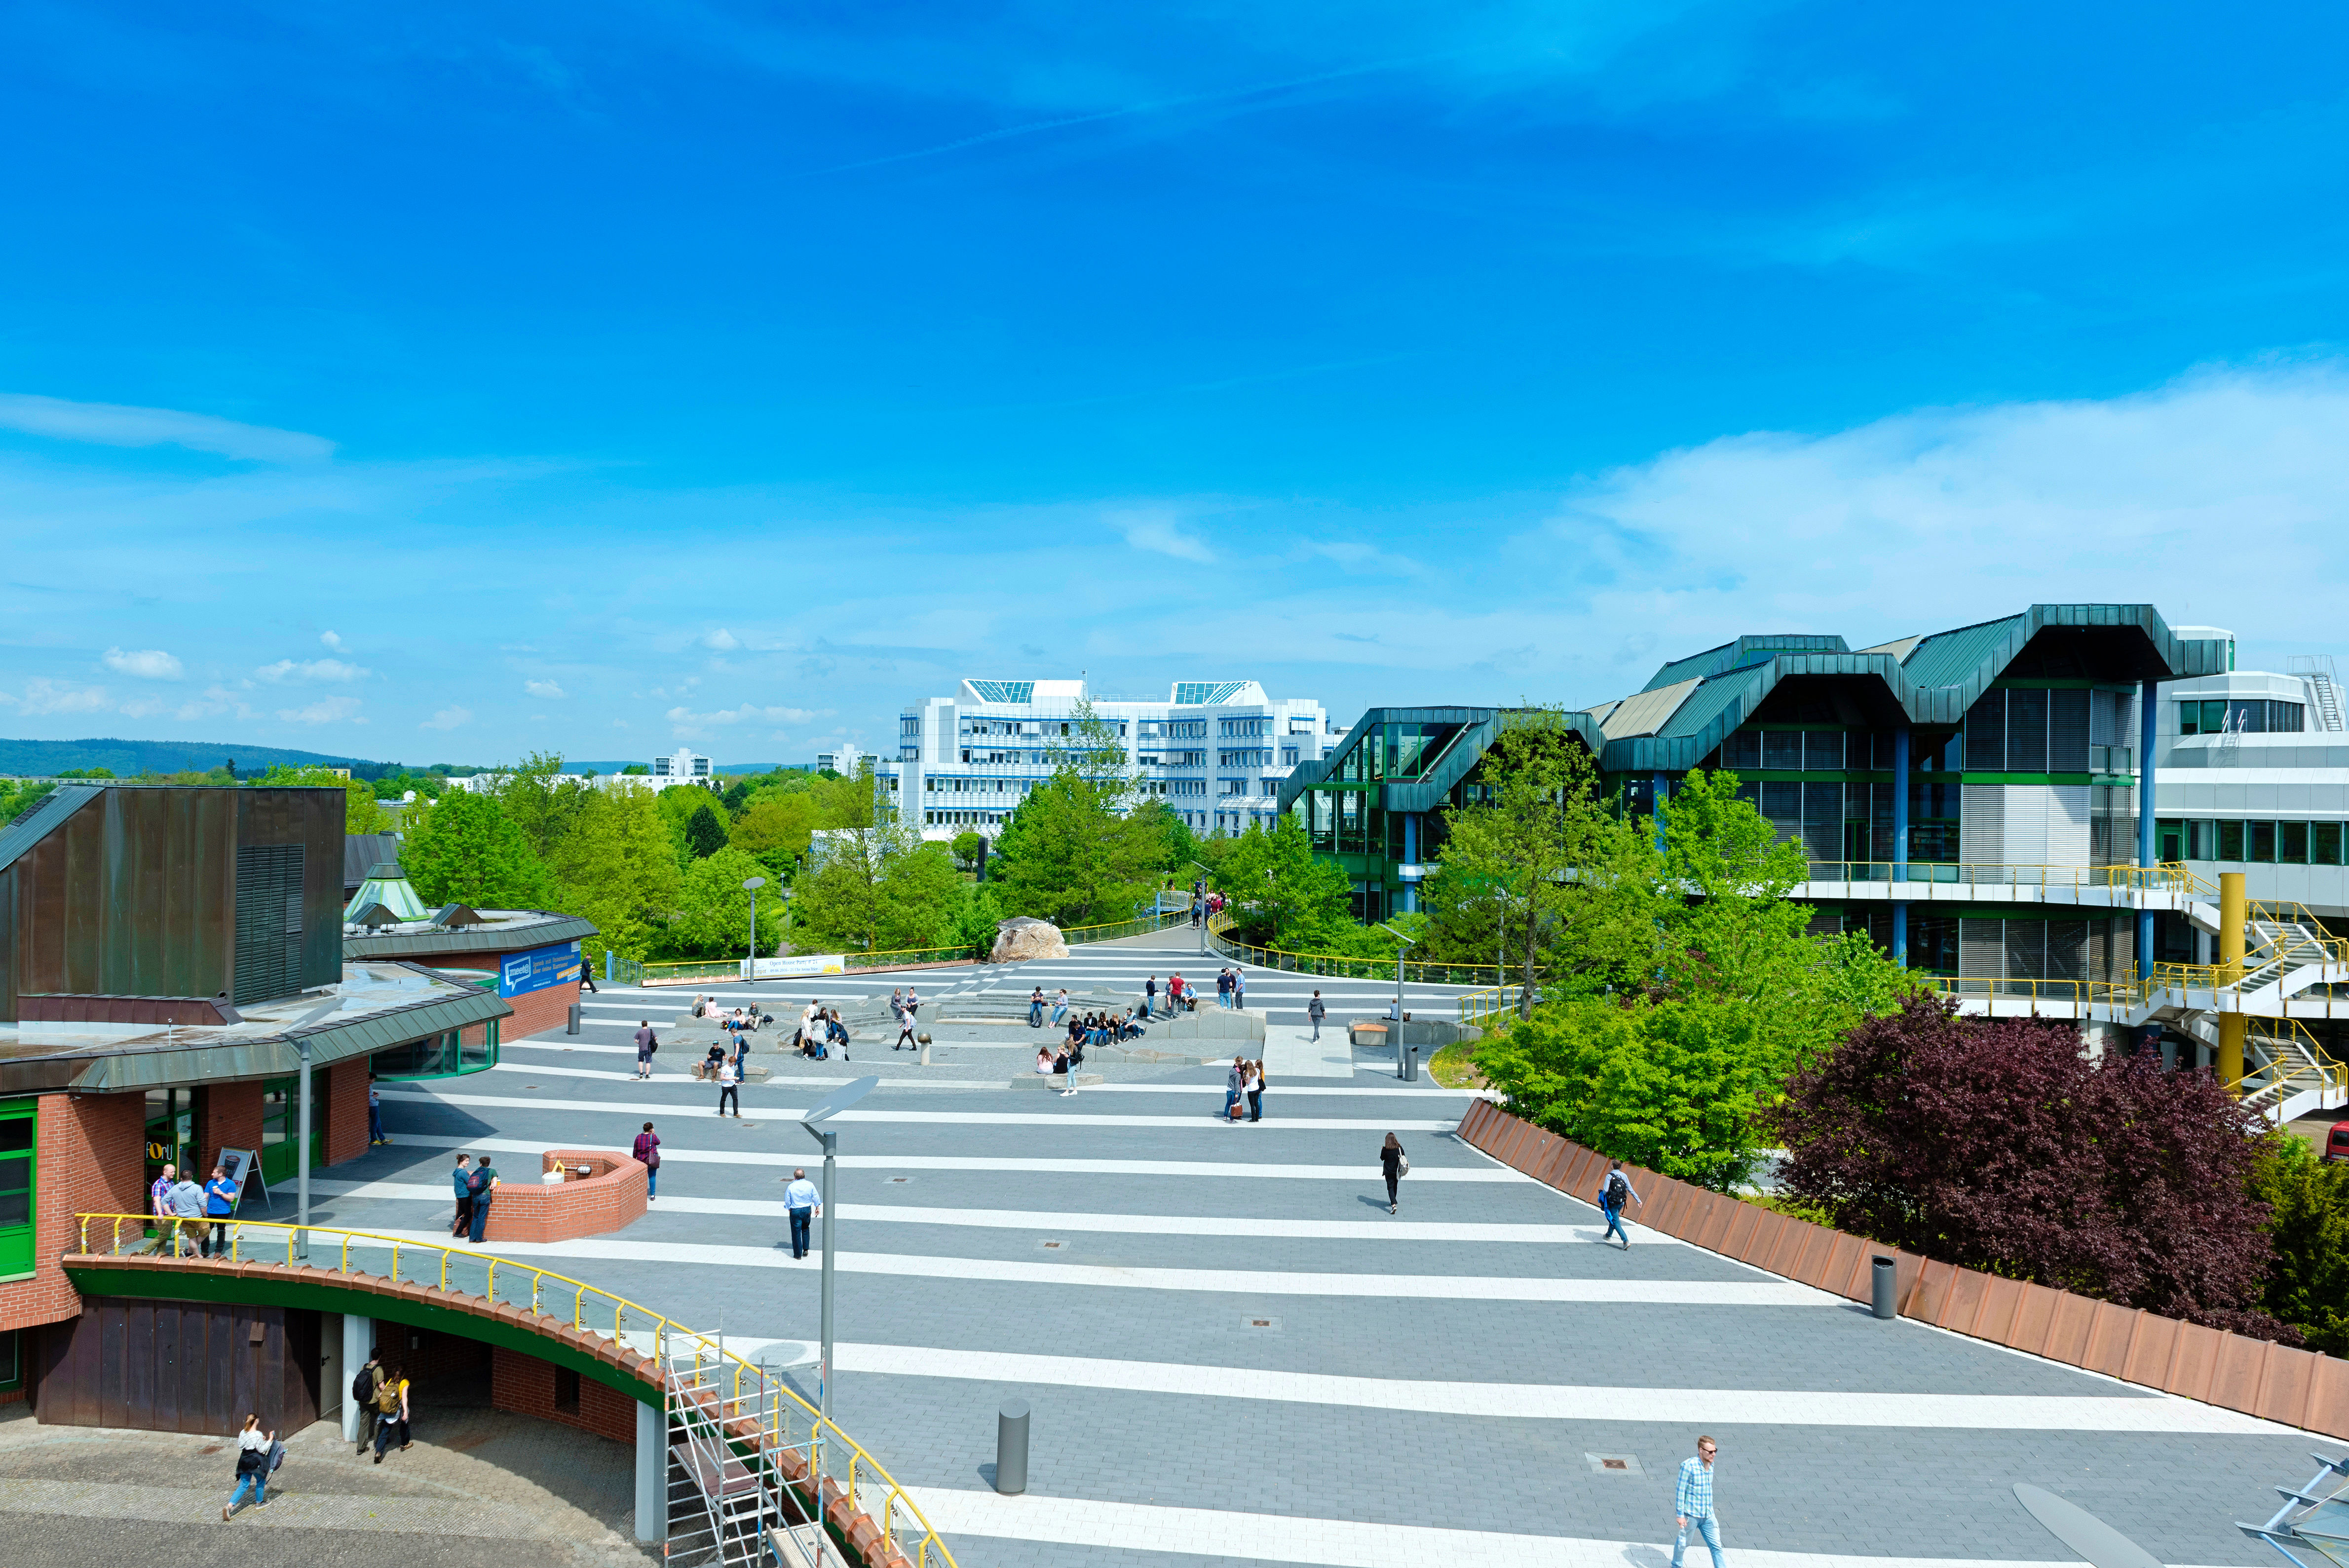
\includegraphics[width=1.2\paperwidth]{unitrier}}
  \begin{frame}
    \maketitle
  \end{frame}
}
    
    %\begin{frame}
       % \frametitle{Inhalt}
		%\tableofcontents
	%\end{frame}
	
%—------------------------------------------------------


\begin{frame}{Ziel: Kleinste Anzahl an Zügen}
	\begin{figure}[ht]
		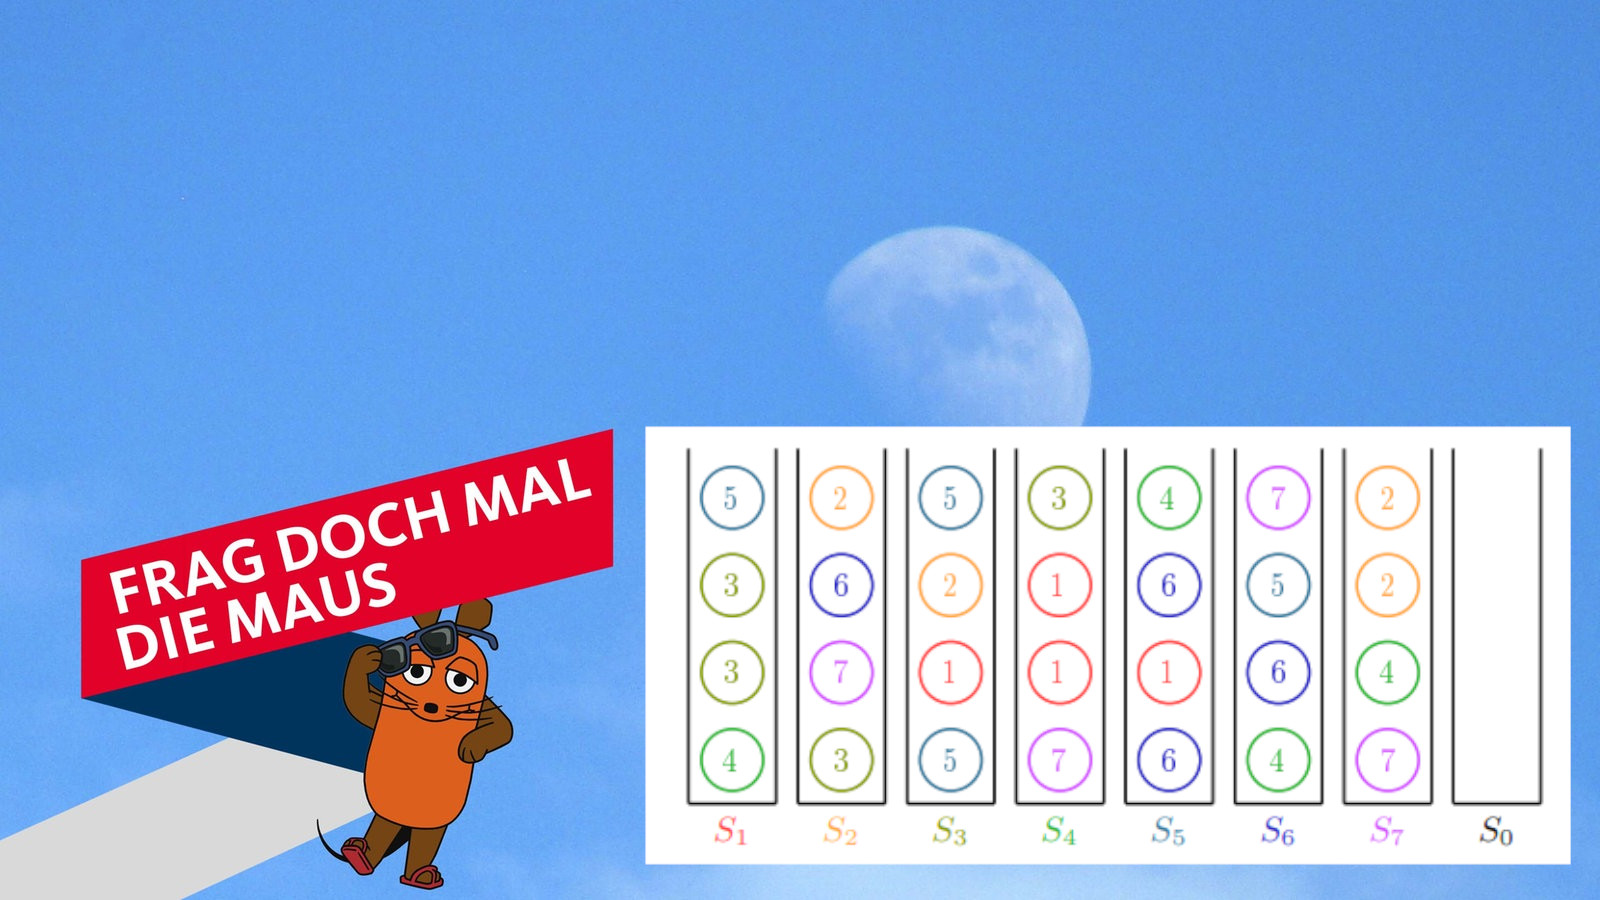
\includegraphics[width=\textwidth]{maus}
    \end{figure}
\end{frame}

\begin{frame}{Idee}
	\begin{itemize}
		\item Konstruktion des Spiels (SCBT) als Graphen 
		\item Reduktion des Problems auf das Feeback Arc Set Problem (FAS)
		\item FAS ist NP-vollständig, somit auch SCBT
	\end{itemize}
\end{frame}

\begin{frame}{Related Work}
	\begin{itemize}
		\item Konstruktion des Spiels (SCBT) als Graphen 
		\item Reduktion des Problems auf das Feeback Arc Set Problem (FAS)
		\item FAS ist NP-vollständig, somit auch SCBT
	\end{itemize}
\end{frame}



\begin{frame}{}
  \centering \Huge
  \emph{Fin}
\end{frame}


	
    	
    	
    	
\end{document}
